\documentclass[12pt,a4paper]{report}
\usepackage[utf8]{inputenc}
\usepackage{parskip}
\usepackage{pdfpages}
\usepackage{amsmath}
\usepackage{url}

\usepackage{graphicx}
\graphicspath{ {./plan_images/} }

\title{Outline and Context Survey}
\author{190005675}
\date{}

\begin{document}

\maketitle
\newpage

\includepdf[pages=-]{content.pdf}

\chapter*{Context Survey}
\section*{Background}
With the climate crisis, there has been a big push from many facets of society to reduce car usage~\cite{CHAPMAN2007354}. Encouraging more people to cycle over short distances instead of driving would be a big step towards reaching that goal. A study by Sloman et al. suggests that investment in cycling leads to increased cycle levels~\cite{Sloman2009}. Many cities and towns have invested money into creating new cycling infrastructure, such as cycle paths alongside roads or standalone cycleways. Public budgets are always squeezed, so it is important to prioritise infrastructure improvements in the places where they would have the most impact. This project aims to investigate how we can determine where those most impactful places will be by analysing the street map of an area.

\section*{Graph Theory}
Street maps can be considered as a type of graph, with nodes being locations on the map and edges being roads and paths which connect the locations. If we consider the subgraph which only consists of cycle-friendly edges, it is possible that there are areas which are isolated from the rest of the graph (i.e. there are no connecting edges between the isolated area and other parts of the graph). Our problem could potentially benefit from many existing graph algorithms.

\subsection*{Connectivity}
Connectivity of a graph is defined as the minimum number of vertices that need to be removed to separate the remaining nodes into two or more isolated subgraphs~\cite{citeulike:395714}. Figure \ref{fig:connectivity4} shows a 4-connected graph; to separate the graph into two isolated subgraphs, the minimum number of vertices that need to be removed is 4. For example, after removing the two left-most vertices and the two right-most vertices, we obtain two disconnected subgraphs, each of which consists of one vertex. 

\begin{figure}[ht]
\centering
\includegraphics[width=0.3\textwidth]{plan_images/connectivity.png}
\caption{A 4-connected graph\protect\footnotemark}
\label{fig:connectivity4}
\end{figure}

\footnotetext{\url{https://en.wikipedia.org/wiki/K-vertex-connected_graph}}

The more connected the cycle-friendly subgraph is, the easier it is to get around the area with bicycles. An intuition to improve the cycle infrastructure would be to add paths that would increase the connectedness of the graph.

\subsection*{Graph traversal}
We could also identify isolated components by exploring the graph. Running a search algorithm from a node will tell us all the reachable nodes from that point. Any nodes in the graph which are not reachable are isolated from this node. Therefore, running search algorithms from each unvisited node will yield the set of isolated components. 

Breadth-first search (BFS) and depth-first search (DFS) are common examples of search algorithms. BFS works by visiting each node in turn, starting with a closest nodes to origin and keeping the unvisited neighbours in a queue. DFS runs in the same way, except it uses a stack, resulting in each branch being explored in full, one at a time. 

\subsection*{Shortest path}
In order to measure the cost of cycling, we can look at the cost of the shortest paths. There are many algorithms for finding the shortest paths between nodes in a graph, perhaps the most famous of which is Dijkstra's shortest path algorithm~\cite{dijkstra1959note}. It takes a starting point and works out the shortest path to all other reachable nodes. Consider the graph in Figure \ref{fig:dijkstra_example}~\cite{abba2022}, we can use Dijkstra's algorithm to find the shortest distance from node A to every other node. During the process, we would keep a priority queue, which stores the shortest distance (so far) to a node from node A, with the smallest distance being at the front of the queue. After visiting the node A, the priority queue would look like this:
\[C=2, B=4, D=\infty, E=\infty\]

\begin{figure}[ht]
\centering
\includegraphics[width=0.5\textwidth]{plan_images/dijkstra.png}
\caption{An undirected graph taken from freeCodeCamp~\cite{abba2022}}
\label{fig:dijkstra_example}
\end{figure}

This is because the shortest distance from A to B is 4, from A to C is 2. Then we choose a new unvisited node from the front of the priority queue, in this case, C. After visiting the node C, we can update the priority queue:
\[B=3, D=\infty, E=\infty\]

C is now visited, so it is removed from the priority queue. Since $2+1 \leq 4$, the shortest distance between AB is updated to be 3. The next node to be visited is B, which is at the front of the priority queue. After visiting B, we have:
\[E=5, D=6\]

And after visiting E, we have:
\[D=6\]

Finally, D is visited and there are no unvisited nodes left. We have computed that the shortest distance from A to every other node:
\[B=3, C=2, D=6, E=5\]

Another famous graph algorithm is Prim's algorithm, which finds the minimum spanning tree for a weighted undirected graph. The minimum spanning tree of a graph is defined to be the tree with the minimum total edge weights which connects all vertices~\cite{Pettie2008}. An example of a minimum spanning tree is shown in Figure \ref{fig:mst_example}. In our task of improving the cycling infrastructure, we can use it to identify the paths that connect all areas with lowest total distance and improve the graph based on this metric.

\begin{figure}[ht]
\centering
\includegraphics[width=0.5\textwidth]{plan_images/MST.png}
\caption{A minimum spanning tree example\protect\footnotemark}
\label{fig:mst_example}
\end{figure}

\footnotetext{\url{https://en.wikipedia.org/wiki/Minimum_spanning_tree}}

\section*{Related Work}
\subsection*{OpenStreetMap}
OpenStreetMap~\cite{OpenStreetMap} is an open, user-generated map database. It is licensed under the Open Data Commons Open Database License\footnote{\url{https://opendatacommons.org/licenses/odbl/}}. There are four types of data in OSM~\cite{9119753}:
\begin{itemize}
    \item A node, which is a location on the Earth's surface
    \item A way, which is a list of nodes representing roads and objects (buildings) along the road
    \item A relation, which specifies the association among objects
    \item A tag, which is a key-value pair regarding information about an object
\end{itemize}

Figure \ref{fig:osm_sta} shows the map of St Andrews in CyclOSM\footnote{\url{https://www.cyclosm.org/#map=16/56.3396/-2.8003/cyclosm}}, a bicycle map based on OpenStreetMap. It highlights bicycle infrastructure such as cycleways, and it includes information about highways such as speed limits. Ferster et al. \cite{doi:10.1080/15568318.2018.1519746} compared OSM data against municipal open data in six Canadian cities and concluded that OSM data was more extensive and detailed.

\begin{figure}[ht!]
\centering
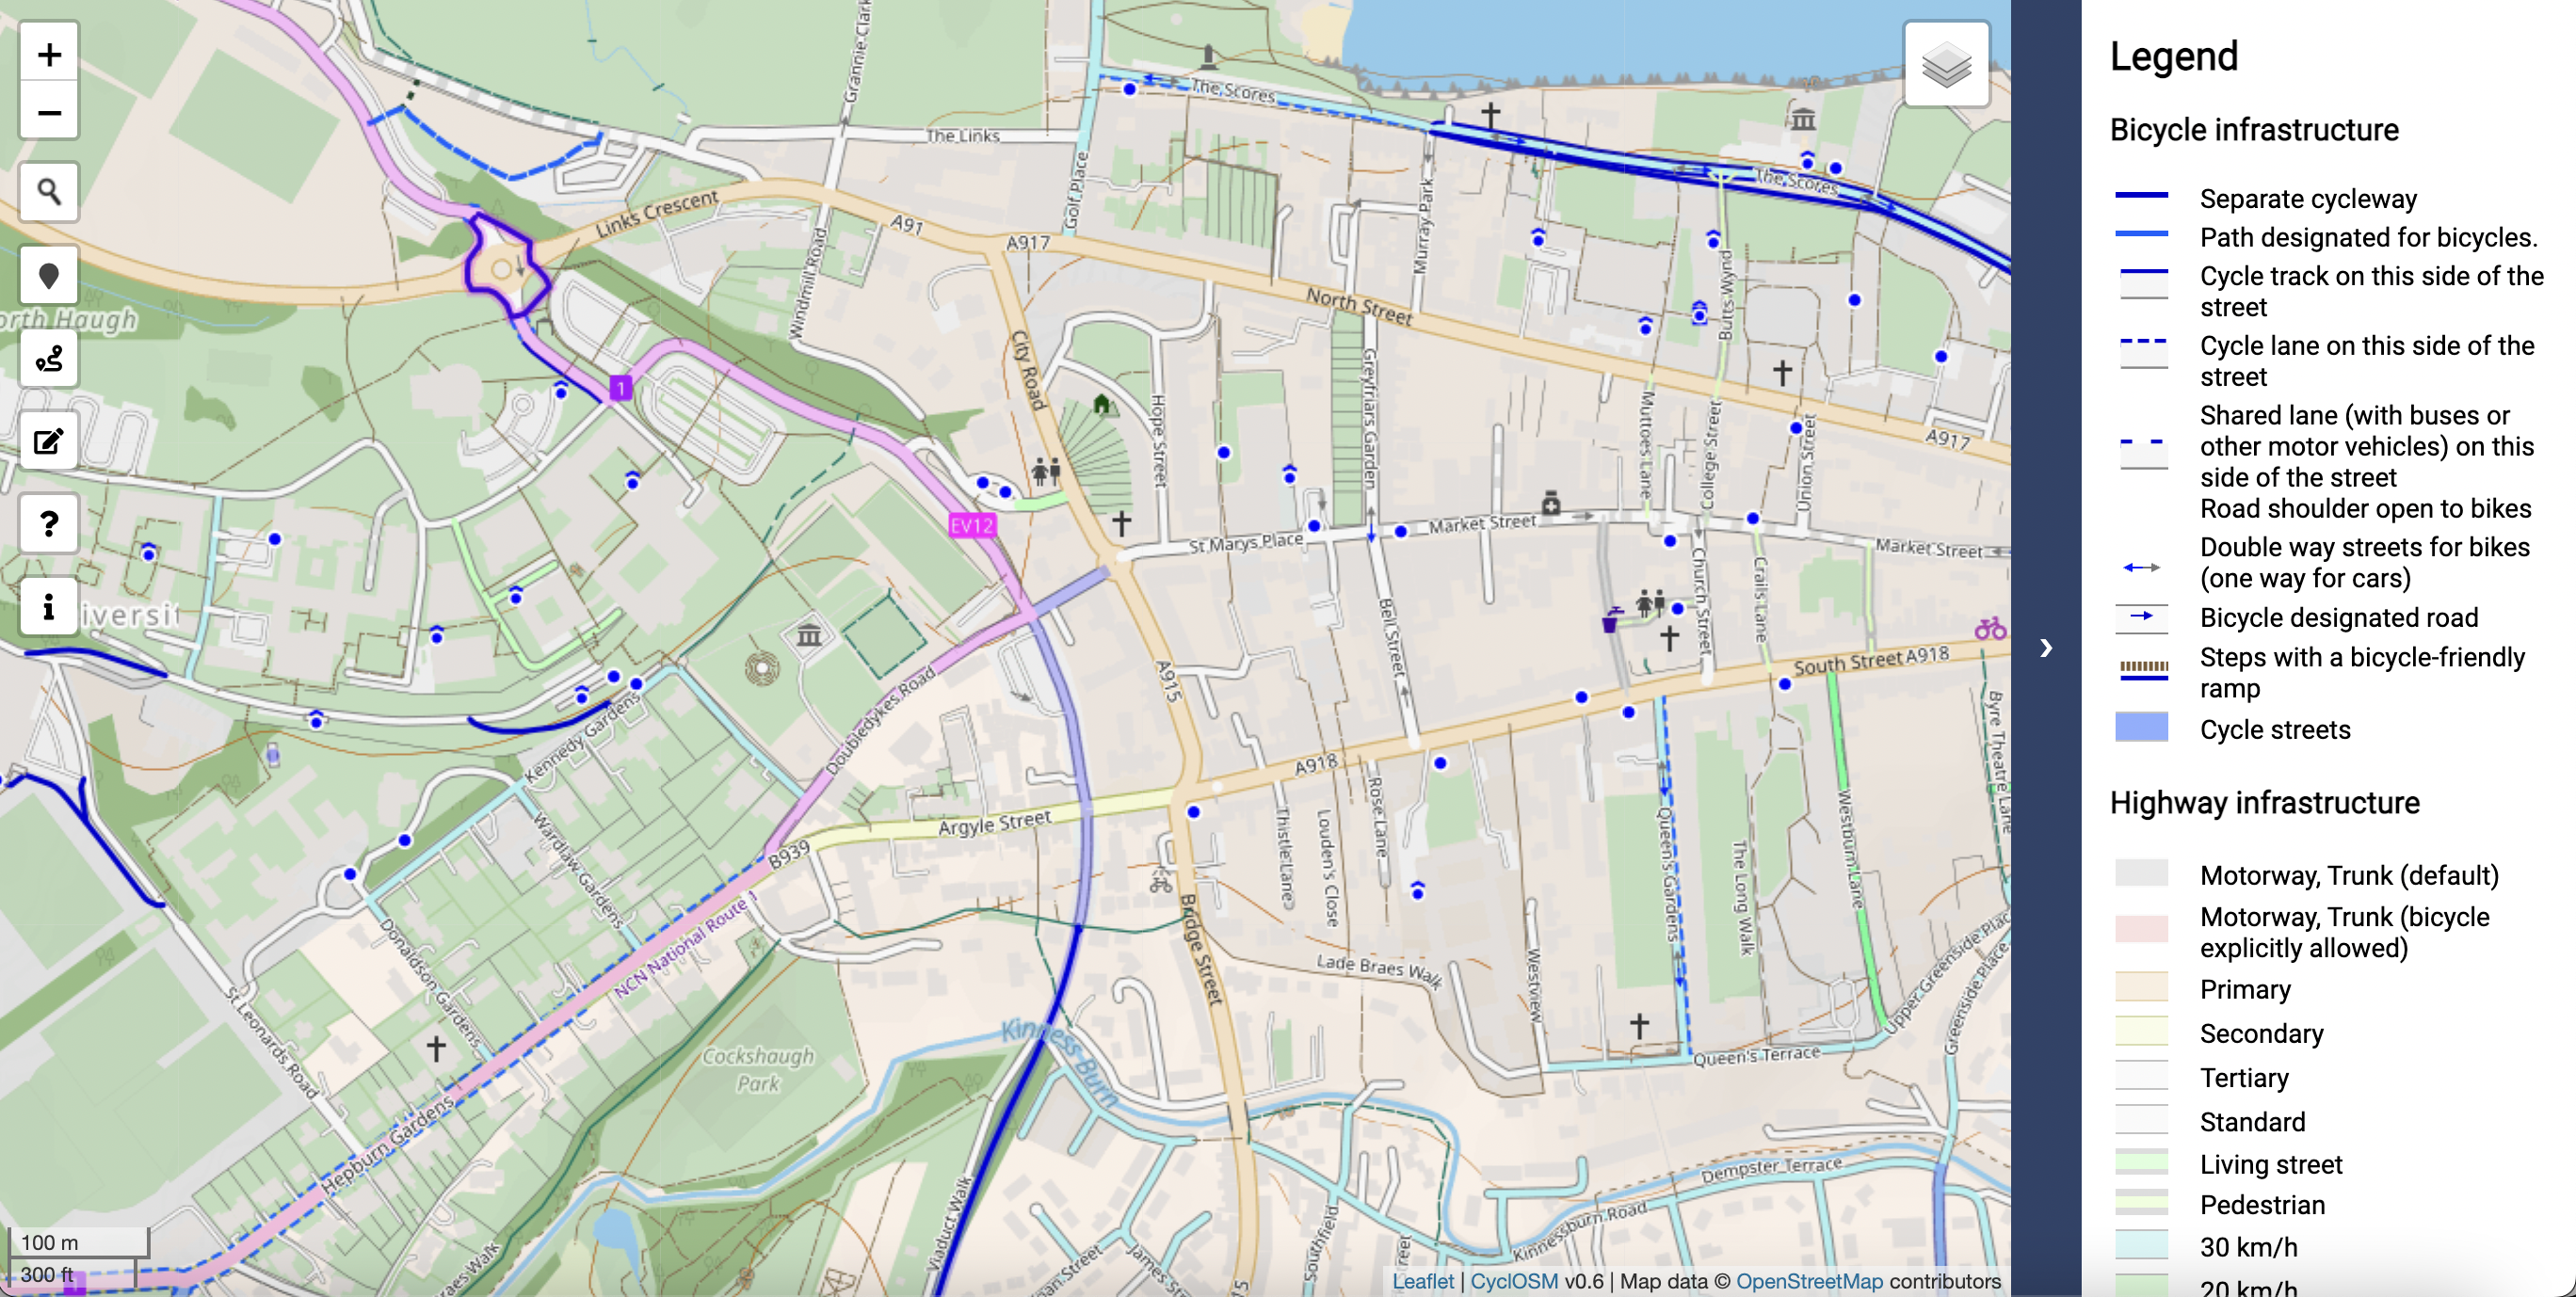
\includegraphics[width=1\textwidth]{plan_images/osm.png}
\caption{CyclOSM of St Andrews}
\label{fig:osm_sta}
\end{figure}

\begin{figure}[ht!]
\centering
\includegraphics[width=1\textwidth]{plan_images/googlemap.png}
\caption{Google map of St Andrews}
\label{fig:google_sta}
\end{figure}

There are other maps that can be used to show bike lanes. For example, Google Maps\footnote{\url{https://www.google.com/maps}} is a widely used map. More than 1 billion people use it every month~\cite{ethan2019}, and by 2018 it supported 40 languages~\cite{yamagami2018}. It makes use of machine learning techniques to remove fake content and help keep the map accurate~\cite{gupta2023}. It also provides a good user interface. Figure \ref{fig:google_sta} shows the map of St Andrews in Google Maps in the Cycling layer.

One disadvantage of Google Maps is that it is not open data. On the other hand, OpenStreetMap is open data and it provides much more detailed information regarding bicycle infrastructure. The OpenStreetMap website\footnote{\url{https://www.openstreetmap.org/}} allows users to query features at any point on the map. Figure \ref{fig:feature_query} shows an example of queried features. Details of each feature can be viewed by clicking the blue text. For example, ``Viaduct Walk" is a link to the information page of Viaduct Walk (Figure \ref{fig:cycleway_query}). It contains a series of tags which specify useful information such as the type of the road, whether pedestrians are allowed and whether it is one-way. It also contains a list of nodes which are on the path. Such information can be helpful for deciding whether a road is cycle-friendly.

\begin{figure}[ht]
\centering
\includegraphics[width=0.8\textwidth]{plan_images/feature.png}
\caption{Querying features in OpenStreetMap}
\label{fig:feature_query}
\end{figure}

\begin{figure}[ht]
\centering
\includegraphics[width=0.8\textwidth]{plan_images/cycleway.png}
\caption{Details of Viaduct Walk}
\label{fig:cycleway_query}
\end{figure}

\subsection*{Applications of Graph Theory}
Since we can model street maps as graphs, it would be helpful to study how graph theory has been applied to other transportation problems. Derrible and Kennedy~\cite{derrible2011} described the history of graph theory with respect to transportation networks, paying particular note to the development of indicators describing the properties of transportation networks. Erath et al.~\cite{erath2009} studied modern measures of the efficiency of transport metrics where they compared cost in the network against the straight-line distance, and showed that parts of the Swiss road network have reached growth limits, where it is hard to improve them any more owing to spatial limitations. Zargham et al.~\cite{zarghami2020} used spanning trees to quantify network reliability, another measure that may be of relevance to cyclists so they can be confident of an alternative route should there be any roadworks.

\subsection*{Applications of Prim's Algorithm}
There are many applications of Prim's algorithm. Wang et al.~\cite{wang2018} developed an algorithm based on Prim's algorithm and used it to identify natural disasters in isolated areas. Fitina et al.~\cite{fitina} discussed applying Prim's algorithm in the context of tourism in Papua New Guinea, in order to reduce the expense of travelling between the islands. Iqbal et al.~\cite{iqbal2017} used Prim's algorithm to optimize the planning of fiber optic cables to reduce the costs. We can see that Prim's algorithm is often used to find the most efficient overall routes, and we would like to improve these routes when building new cycling infrastructure. 

\subsection*{Software and Tools}
As discussed before, graph algorithms can be helpful for our task. Some libraries provide efficient graph-theory algorithms, such as \texttt{python-igraph}\footnote{\url{https://python.igraph.org/en/stable/}} in Python and \texttt{JGraphT}\footnote{\url{https://jgrapht.org/}} in Java.

\texttt{python-igraph}~\cite{csardi2005} is an open source library for analysing graphs. It provides methods such as traversing a graph, finding the shortest paths, finding a minimum spanning tree, and computing the edge connectivity and vertex connectivity of a graph. It is also possible to visualize the graphs, either with \texttt{matplotlib}\footnote{\url{https://matplotlib.org/}} or with its default image viewer.

\texttt{JGraphT}~\cite{jgrapht} is a Java library for graph theory algorithms. It also comes with Python bindings, \texttt{Python-JGraphT}\footnote{\url{https://pypi.org/project/jgrapht/}}. Similar to \texttt{python-igraph}, it contains algorithms on shortest paths, connectivity and minimum spanning trees. It provides more methods for graph traversals than \texttt{python-igraph}. In addition to breadth-first search, depth-first search and random walk traversal provided in \texttt{python-igraph}, it also includes other types of traversals such as topological order traversal.

\bibliographystyle{plain}
\addcontentsline{toc}{chapter}{Bibliography}
\bibliography{plan_refs}

\chapter*{Work Plan}
\textbf{(Week 1) 29 May - 4 June}\\
Background research and context survey.

\textbf{(Week 2) 5 June - 11 June}\\
Write up the context survey.

\textbf{(Week 3) 12 June - 18 June}\\
Analyse the data and preprocess the OpenStreetMap data. Decide on a set of heuristics for cycle-friendliness. Select and learn a graph analysis tool.

\textbf{(Week 4) 19 June - 25 June}\\
Implement a script that can suggest paths to improve cycling infrastructure based on St Andrews OSM data and one of the heuristics.

\textbf{(Week 5) 26 June - 2 July}\\
Prepare for interim demo. Refine the code and investigate other heuristics.

\textbf{(Week 6) 3 July - 9 July}\\
Write up design and implementation chapters of the final report.

\textbf{(Week 7) 10 July - 16 July}\\
Apply the technique to another area and analyse differences between that area and St Andrews.

\textbf{(Week 8) 17 July - 23 July}\\
Time allocated for resolving any unexpected difficulties that arise.

\textbf{(Week 9) 24 July - 30 July}\\
Write up evaluation chapter of the final report.

\textbf{(Week 10) 31 July - 6 August}\\
Finalise the evaluation and submit full draft to supervisor.

\textbf{(Week 11) 7 August - 13 August}\\
Prepare final report and supporting materials for submission.

\end{document}
